\documentclass[
  digital,     %% The `digital` option enables the default options for the
               %% digital version of a document. Replace with `printed`
               %% to enable the default options for the printed version
               %% of a document.
%%  color,       %% Uncomment these lines (by removing the %% at the
%%               %% beginning) to use color in the printed version of your
%%               %% document
  oneside,     %% The `oneside` option enables one-sided typesetting,
               %% which is preferred if you are only going to submit a
               %% digital version of your thesis. Replace with `twoside`
               %% for double-sided typesetting if you are planning to
               %% also print your thesis. For double-sided typesetting,
               %% use at least 120 g/m² paper to prevent show-through.
  nosansbold,  %% The `nosansbold` option prevents the use of the
               %% sans-serif type face for bold text. Replace with
               %% `sansbold` to use sans-serif type face for bold text.
  nocolorbold, %% The `nocolorbold` option disables the usage of the
               %% blue color for bold text, instead using black. Replace
               %% with `colorbold` to use blue for bold text.
  lof,         %% The `lof` option prints the List of Figures. Replace
               %% with `nolof` to hide the List of Figures.
  lot,         %% The `lot` option prints the List of Tables. Replace
               %% with `nolot` to hide the List of Tables.
]{fithesis4}
%% The following section sets up the locales used in the thesis.
\usepackage[resetfonts]{cmap} %% We need to load the T2A font encoding
\usepackage[T1,T2A]{fontenc}  %% to use the Cyrillic fonts with Russian texts.
\usepackage[
  main=english, %% By using `czech` or `slovak` as the main locale
                %% instead of `english`, you can typeset the thesis
                %% in either Czech or Slovak, respectively.
  english, czech, slovak %% The additional keys allow
]{babel}        %% foreign texts to be typeset as follows:
%%
%%   \begin{otherlanguage}{german}  ... \end{otherlanguage}
%%   \begin{otherlanguage}{russian} ... \end{otherlanguage}
%%   \begin{otherlanguage}{czech}   ... \end{otherlanguage}
%%   \begin{otherlanguage}{slovak}  ... \end{otherlanguage}
%%
%% For non-Latin scripts, it may be necessary to load additional
%% fonts:
\usepackage{paratype}
\def\textrussian#1{{\usefont{T2A}{PTSerif-TLF}{m}{rm}#1}}
%%
%% The following section sets up the metadata of the thesis.
\thesissetup{
    date        = \the\year/\the\month/\the\day,
    university  = mu,
    faculty     = fi,
    type        = bc,
    department  = Department of Visual Computing,
    author      = Bruno Petrus,
    gender      = m,
    advisor     = {doc. RNDr. Martin Maška, Ph.D.},
    title       = {Segmentation of Membrane-Stained Cells in Image Data of Organoids},
    TeXtitle    = {Segmentation of Membrane-Stained Cells in Image Data of Organoids},
    keywords    = {keyword1, keyword2, ...},
    TeXkeywords = {keyword1, keyword2, \ldots},
    abstract    = {%
      This is the abstract of my thesis, which can

      span multiple paragraphs.
    },
    thanks      = {%
      These are the acknowledgements for my thesis, which can

      span multiple paragraphs.
    },
    bib         = bibliography.bib,
    %% Remove the following line to use the JVS 2018 faculty logo.
    facultyLogo = fithesis-fi,
}
\usepackage{makeidx}      %% The `makeidx` package contains
\makeindex                %% helper commands for index typesetting.
%% These additional packages are used within the document:
\usepackage{paralist} %% Compact list environments
\usepackage{amsmath}  %% Mathematics
\usepackage{amsthm}
\usepackage{amsfonts}
\usepackage{url}      %% Hyperlinks
\usepackage{markdown} %% Lightweight markup
\usepackage{listings} %% Source code highlighting
\lstset{
  basicstyle      = \ttfamily,
  identifierstyle = \color{black},
  keywordstyle    = \color{blue},
  keywordstyle    = {[2]\color{cyan}},
  keywordstyle    = {[3]\color{olive}},
  stringstyle     = \color{teal},
  commentstyle    = \itshape\color{magenta},
  breaklines      = true,
}
\usepackage{floatrow} %% Putting captions above tables
\floatsetup[table]{capposition=top}
\usepackage[babel]{csquotes} %% Context-sensitive quotation marks

%% Specify new commands
\newcommand*{\R}{\ensuremath{\mathbb{R}}}
\newcommand*{\Z}{\ensuremath{\mathbb{Z}}}

\begin{document}
%% The \chapter* command can be used to produce unnumbered chapters:
\chapter*{Introduction}
%% Unlike \chapter, \chapter* does not update the headings and does not
%% enter the chapter to the table of contents. I we want correct
%% headings and a table of contents entry, we must add them manually:
\markright{\textsc{Introduction}}
\addcontentsline{toc}{chapter}{Introduction}

Theses are rumoured to be \enquote{the capstones of education}, so
I decided to write one of my own. If all goes well, I will soon
have a diploma under my belt. Wish me luck!

\chapter{Theory}

\section{Digital Image}

Our eyesight is arguably one of our most helpful sense for observing the world.
Researchers have developed many tools which help us study the world. I will
begin by formalizing the concept of images so that we can use mathematics
and computer science to describe them.

Essentially we can think of an image as an n-dimensional function $f(x_1, x_2,
..., x_n)$, where $x_1, x_2, .. x_n$ are coordinates inside a spatial plane,
while the function value at those coordinates specifies the magnitude or intensity
of the signal at that point. In most general terms, we can think about images as
functions of type $f:\R^n \rightarrow \R^m$, where $n$ indicates the number of
spatial dimensions and $m$ specifies the number of channels. For example, when
we are talking about two-dimensional greyscale images, $m$ is equal to 1 and $n$ is
equal to 2, while a typical coloured photograph can have more than 3 channels.

In real life, we do not necessarily work with real-valued spatial dimensions and
intensities but only have a finite number of bits. The process of
acquiring images in a finite grid and assigning intensities from a finite
range is called sampling and quantization. In essence, we create a discretized
version of the original signal, which can be represented as an array of values.
If both the coordinates and the intensity are subsets of some discrete and finite set,
we can think of them as a digital image.

\section{Image smoothing}

\section{Edge finding}

In digital image processing, edges typically separate different regions of
interest from each other. They are essential in digital image processing
as they can be used in many workflows --- such as image segmentation and
classification --- to extract various interesting features and regions
from the image.

There is no authoritative definition of an edge, but it can be thought of as a
set of connected pixels that lie on the boundary between two regions
\parencite{gonzalez2002}. Usually, there is a gradient of intensities between two
regions, as can be seen in the Figure \ref{fig:edge_intensities}. It is hard to
define precisely where an edge begins and ends, so the first and the second
derivative of the image is usually calculated and analysed.


\begin{figure}
    \begin{center}
        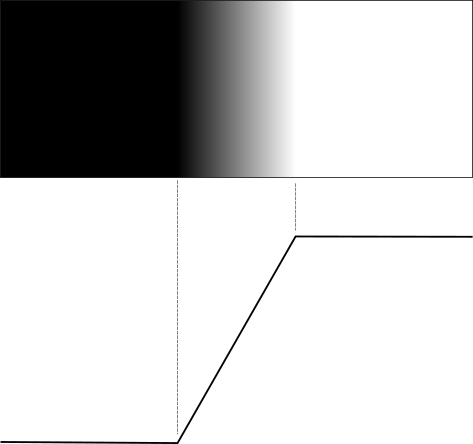
\includegraphics[width=6cm]{resources/inkscape/gradient.png}
    \end{center}
    \caption{Intesity of an image.}
    \label{fig:edge_intensities}
\end{figure}

\subsection{Gradient operators}

The first common way of working out where the edge is located is by looking at
the gradient of the image. The gradient of an image $f(x,y)$ at position $(x,
y)$ is defined as vector
\parencite{gonzalez2002}:
$$\nabla \textbf{f} =
\begin{bmatrix}
    G_x \\
    G_y
\end{bmatrix} =
\begin{bmatrix}
    \dfrac{\partial f}{\partial x}\\[2ex]
    \dfrac{\partial f}{\partial y}
\end{bmatrix}$$
The vector gradient represents the rate of change in the image, and it points in
the direction of the maximum rate of change of intensity. Often just the bare
vector is not of interest; instead, the magnitude of the gradient, denoted as
$\nabla f$, is calculated too. Confusingly enough, sometimes this is also called
the gradient in the literature, but here I will differentiate it using the bold
text. Formally it is defined as:
$$\nabla f = \text{mag}(\nabla \textbf{f}) = \sqrt{G_x^2 + G_y^2}$$
where $G_i$ symbolises the gradient in the $i$ axis.

Now the question is how to calculate the $G_x$ and $G_y$ of some digital image.
It is impossible to calculate the partial derivatives using the standard
definition from mathematical analysis because digital images are discrete; thus,
we must use an approximation. Even though using something like the Sobel filter
is very common, in my prototype, a more basic Prewitt filter will suffice.
\begin{figure}
    \begin{center}
        \begin{tabular}{ |c|c|c| }
            \hline
            -1 & 0 & 1 \\
            \hline
            -1 & \underline{0} & 1 \\
            \hline
            -1 & 0 & 1 \\
            \hline
        \end{tabular}
        \begin{tabular}{ |c|c|c| }
            \hline
            -1 & -1 & -1 \\
            \hline
            0 & \underline{0} & 0 \\
            \hline
            1 & 1 & 1 \\
            \hline
        \end{tabular}
    \end{center}
    \caption{Prewitt horizontal and vertical mask.}
    \label{table:prewitt}
\end{figure}
The horizontal Prewitt filter for 3x3 region looks like in the Figure
\ref{table:prewitt}.
The underlined 0 indicates the centre and the numbers specify weights in the
neighbourhood of a pixel. Summing them all together we arrive at the horizontal or
vertical approximation of the gradient.

TODO image

\subsection{Laplacian operator}

The second common way of finding edges is using the second derivative, or more
precisely using the Laplacian. For a 2D function $f(x, y)$ the Laplacian is
defines as \parencite{gonzalez2002}:

$$\nabla^2 f = \frac{\partial^2 f}{\partial x^2} + \frac{\partial^2 f}{\partial y^2}$$

However, in the context of digital image processing our signal is discrete;
therefore, a discrete approximation is needed. A fairly standard way is to use
the following approach to calculate the partial second derivative in the $x$
axis:
$$\frac{\partial^2 f}{\partial x^2} = f(x + 1, y) + f(x - 1, y) - 2*f(x, y)$$
and similar in the y axis:
$$\frac{\partial^2 f}{\partial y^2} = f(x, y + 1) + f(x, y - 1) - 2*f(x, y)$$
Substituting into the prior definition we get the following approximation:
$$\nabla^2 f = f(x+1, y) + f(x-1, y) + f(x, y+1) + f(x, y-1) - 4*f(x,y)$$
To calculate the Laplacian of an image, this formula is applied on each pixel.

% todo insert an image and description
% todo insert and examplorary image

\begin{figure}
    \begin{center}
        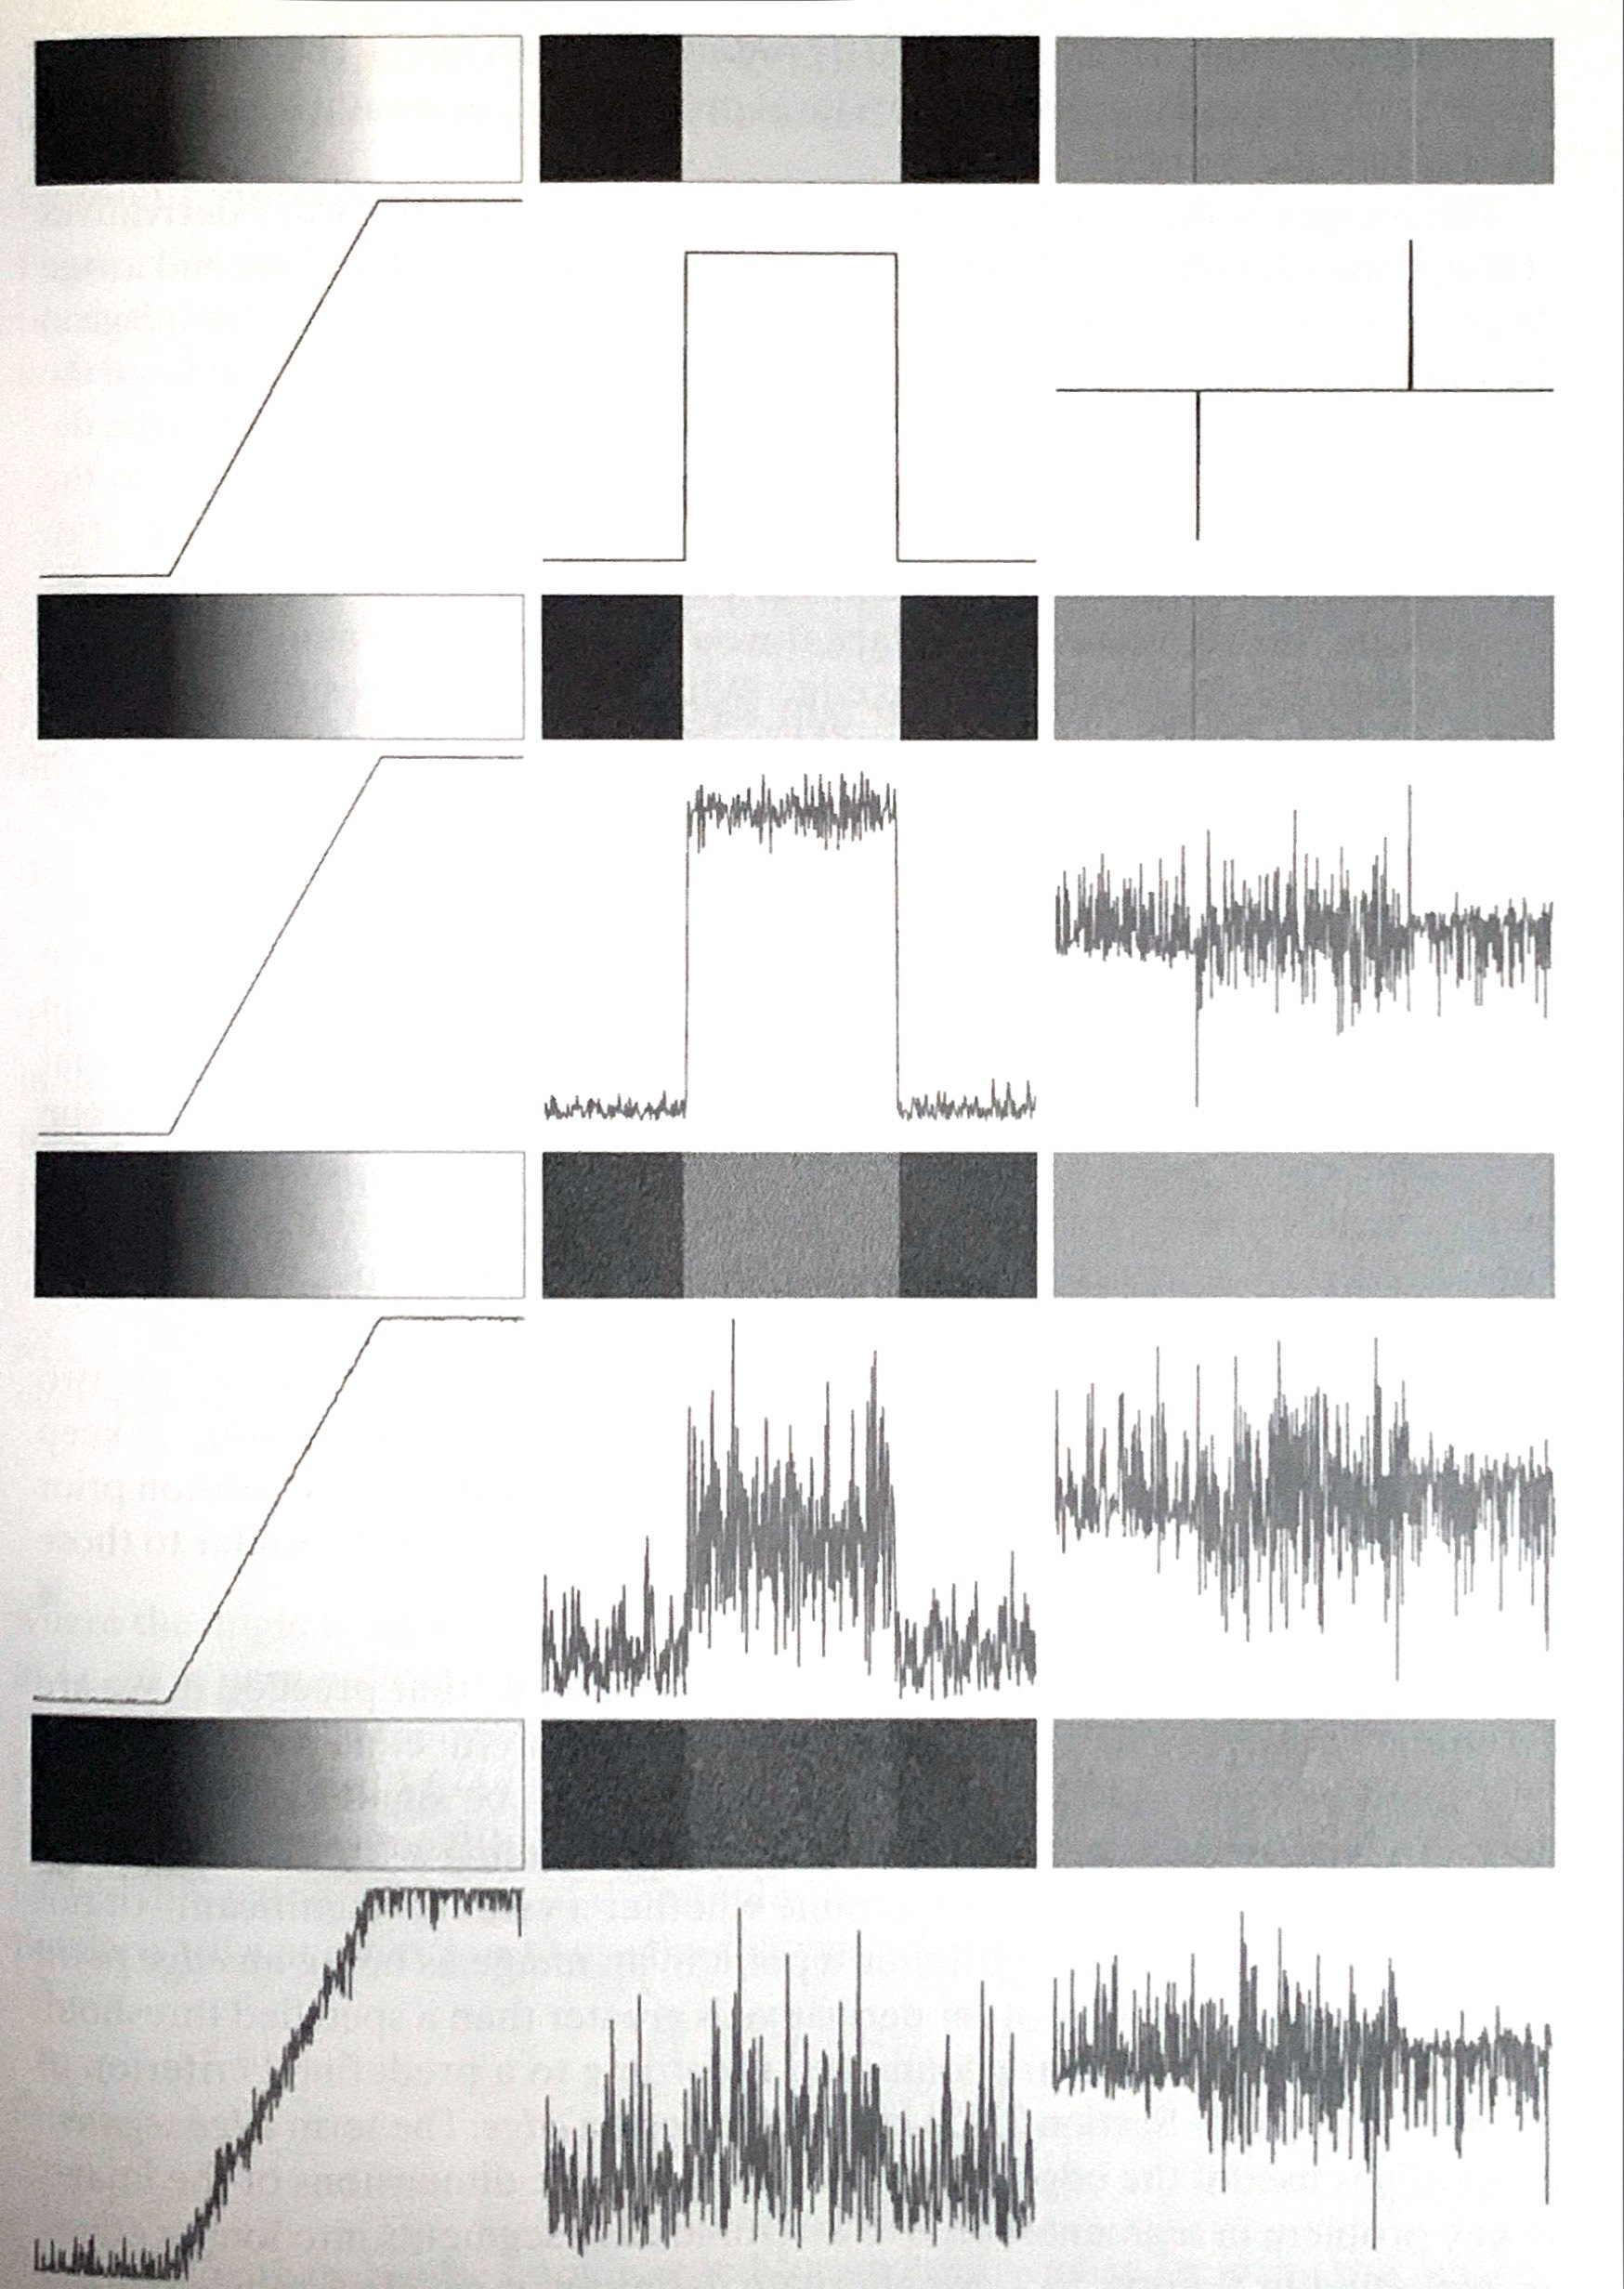
\includegraphics[width=6cm]{"resources/gonzalez_edges_and_noise.jpg"}
    \end{center}
    \caption{Effect of noise on signal \parencite{gonzalez2002}}
    \label{fig:edges_noise}
\end{figure}

One of the disadvantages of this approach is the sensitivity to noise. For
demonstration purposes, the effects will be shown in 1D. In Figure
\ref{fig:edges_noise}, the effect of noise is demonstrated. While the original
signal does not look too destroyed, it is impossible to find the correct
zero-crossings. Therefore we have to help the operator by first smoothing the
image. A common approach is to first use Gaussian smoothing; this is sometimes
called a Laplacian of Gaussian operator or a Mexican hat filer. The idea is that
by averaging, we reduce some of the effects of the noise. The Figure \textbf{TODO}
demonstrates this effect.

Since the Laplacian is based on second derivatives, it has the property that
each edge produces a zero crossing. This can be readily utilised to find edges
inside an image. A simple algorithm is to go through the whole image and check
if a particular pixel at a given position is positive while its neighbours are
negative. If this condition is true, we set this position to white in the
resulting image and black otherwise. This creates an TODO. Here another valuable
property of the zero-crossing algorithm can be seen. The produced edges are
thin, and form closed contours.

\section{Thresholding}

\subsection{Otsu method}

The Otsu thresholding method is a popular technique to determine a threshold
value between two classes (usually the foreground and the background). As such,
it works well if the image has a clear bimodal distribution. The main idea of
this approach is to see the problem of finding the threshold as an optimization
problem, where the inter-class variance of the two classes is to be minimized.
For some threshold $t$ we can define the variance as \parencite{otsu1979}:
$$\sigma^2_W = \sigma^2_0 \omega_0 + \sigma^2_1 \omega_1$$  %todo: whats w?
where the weight $\omega_1$ and $\omega_2$ are the probabilities of the two
classes. It can be shown that minimizing the intra-class variance is the same as
maximizing inter-class variance \parencite{otsu1979}. This idea leads to an
efficient algorithm employed by many image processing libraries, such as
scikit-image.

TODO image and histogram

\subsection{Gradient threshold}

Another useful thresholding method is the gradient threshold algorithm. Unlike
many other thresholding algorithms, it does not purely rely on the analysis of
the image's histogram; instead, the threshold is calculated as a weighted sum of
the image's intensities, where the weights are dictated by the magnitude of the
gradient \cite{pb130}.

The idea is that the background tends to be rather uniform compared to the
object in the foreground; hence, the magnitude of the gradient is the greatest
in the foreground, and the edge separating it from the background. That can be
utilized by using the magnitude as the weight in the summing of intensities.
This way the background's intensities play lesser role.

Formally the threshold $a$ is defined as:
$$a = \sum_{u, v} I(u, v) \frac{|\nabla I(u, v)|}{\sum_{i, j} |\nabla(i,j)|}$$
where $I(i, j)$ stands for the image intensity at the $(i, j)$ position.

\begin{figure}
    \begin{center}
        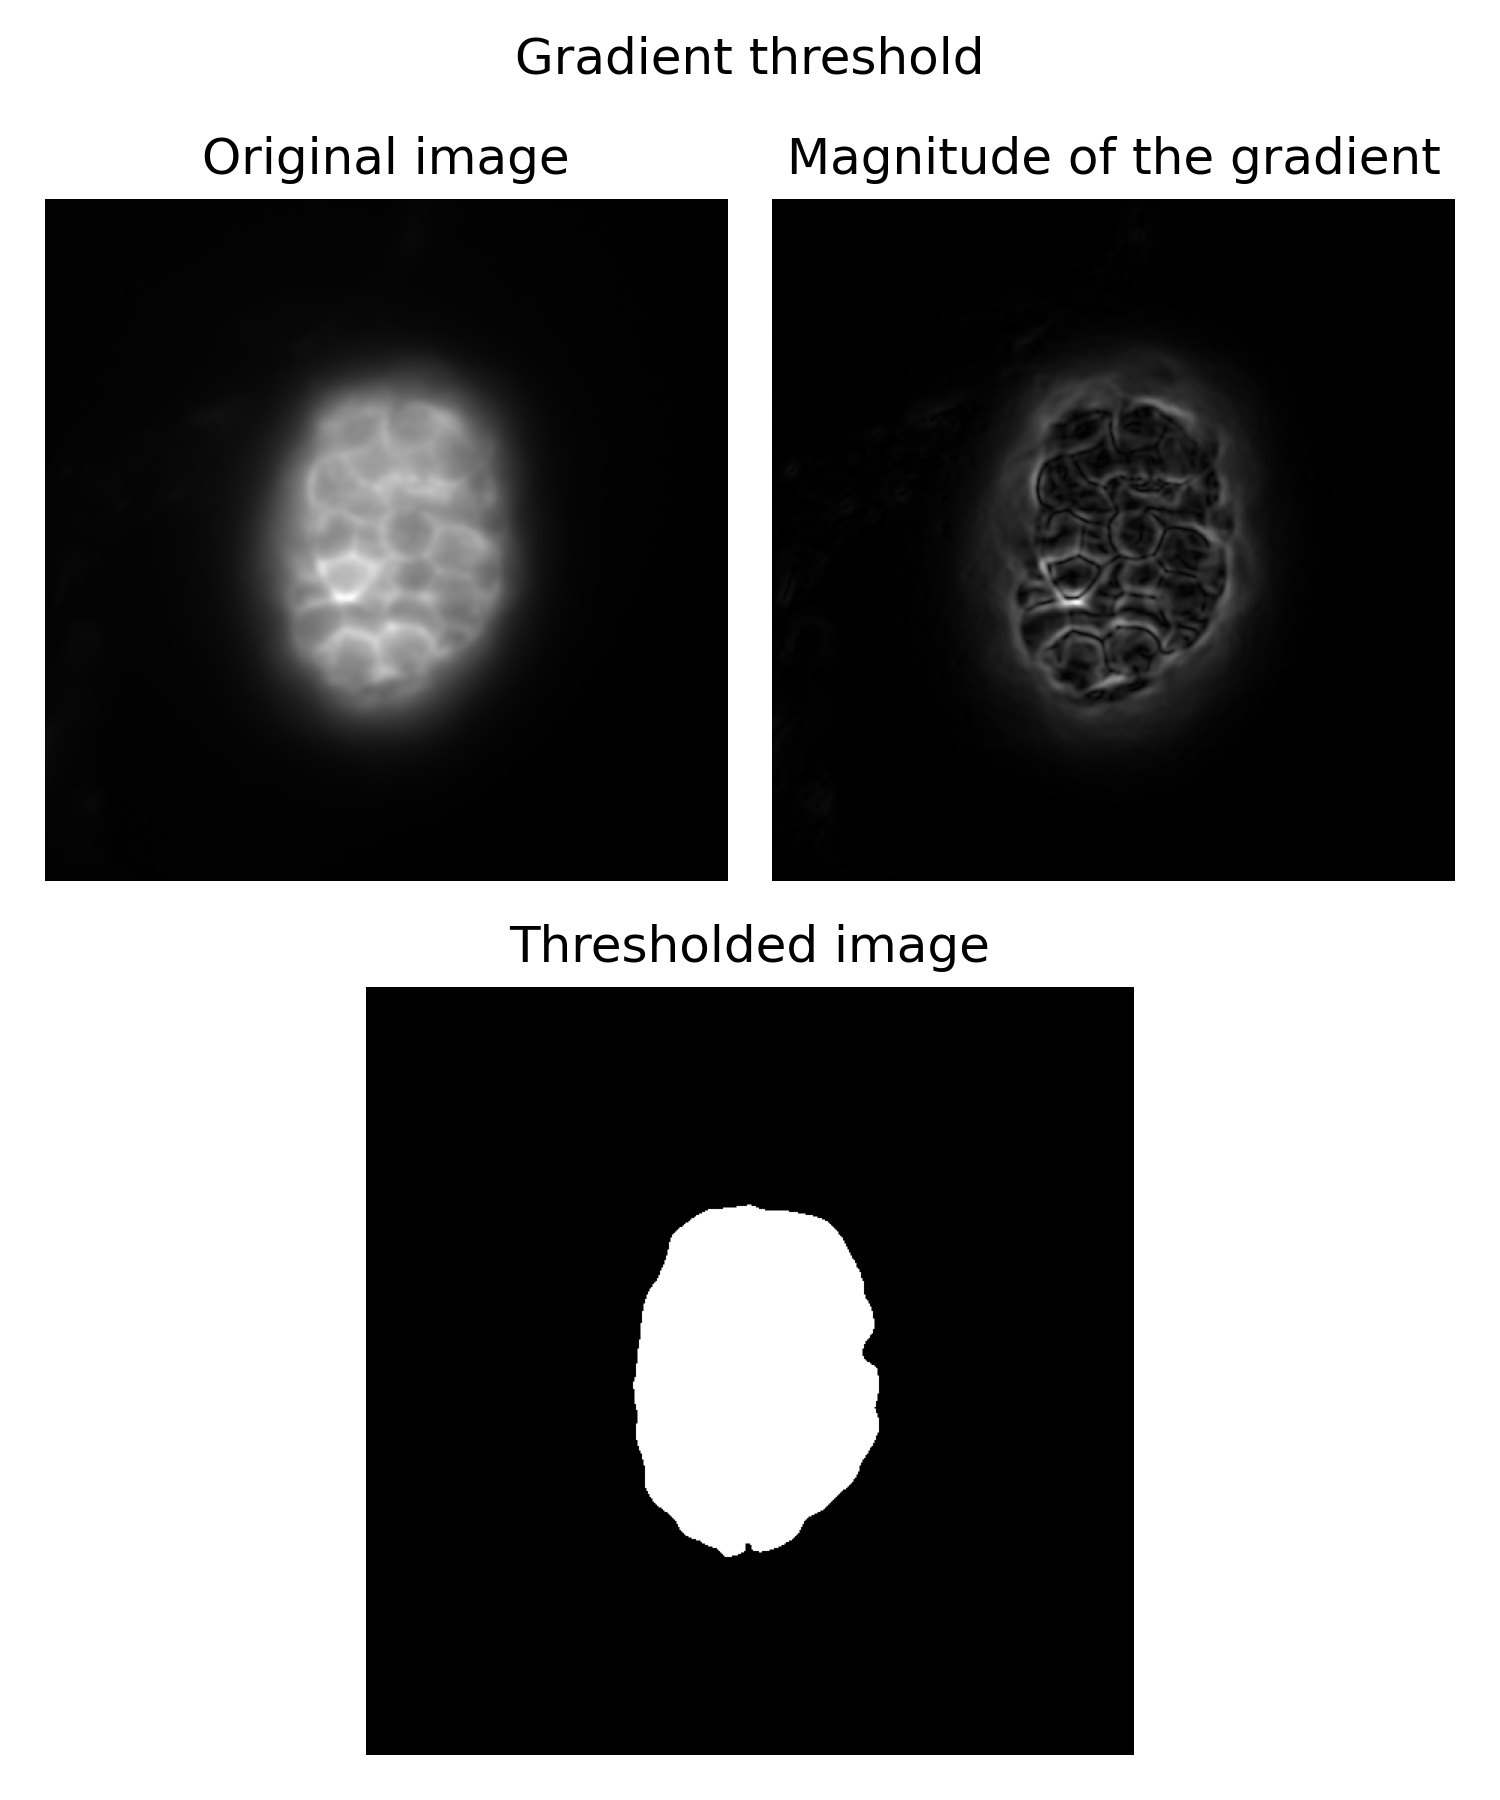
\includegraphics[width=8cm]{"resources/demo-gradient-threshold.png"}
    \end{center}
    \caption{Demo of gradient threshold.}
    \label{fig:demo_grad_thresh}
\end{figure}

In Figure \ref{fig:demo_grad_thresh} an example image is shown. There, the
gradient thresholding algorithm was used to segment the cell from the
background. As can be seen, the magnitude of the gradient is biggest in the
cell; hence, it contributes more to the value of the threshold.

\textbf{TODO: Why this threshold method is useful}

\section{Mathematical morphology}

Mathematical morphology is a tool used to extract various interesting features
from images. The tasks include edge-detecting algorithms, finding convex hulls, and filtering
, just to name a few. In the simplest terms,
mathematical morphology looks at images as sets of numbers and modifies them using structural elements. Those can take many forms, but their shape varies based on the task we are trying
to achieve. The main use of mathematical morphology in this thesis is
to pre- and post-process image data generated by other image processing methods.
First, some basic operations on binary images are described. Note that
this area is vast and still being actively researched, and I will cover only parts which are helpful later in my
prototype.

In this branch of image processing, we look at the images through set theory
instead of looking at images as discrete-valued functions. In this context, an
image is a subset of 2-D integer space $\Z^2$, which can easily be generalized
to more dimensions. Each element of this subset $(x, y)$ represents a present
pixel at those coordinates in the image. In other words, if we look at an image
as an array of rectangular shape, then each foreground pixel's coordinates will
be included in the set representation.

\subsection{Preliminary}
Before we look at the two main operations --- erosion and dilation --- we have to
define two not-so-common operations on sets which are heavily used in
mathematical morphology.

During the following sections, we need to be able to talk about how to create a
reflection of the image around its origin, as is shown in the figure
\ref{fig:morp_refl}. Reflection is formally defined as \parencite{gonzalez2002}:
$$\hat{B} = \{w | w=-b \text{ , for } b \in B\}$$
\begin{figure}
    \begin{center}
        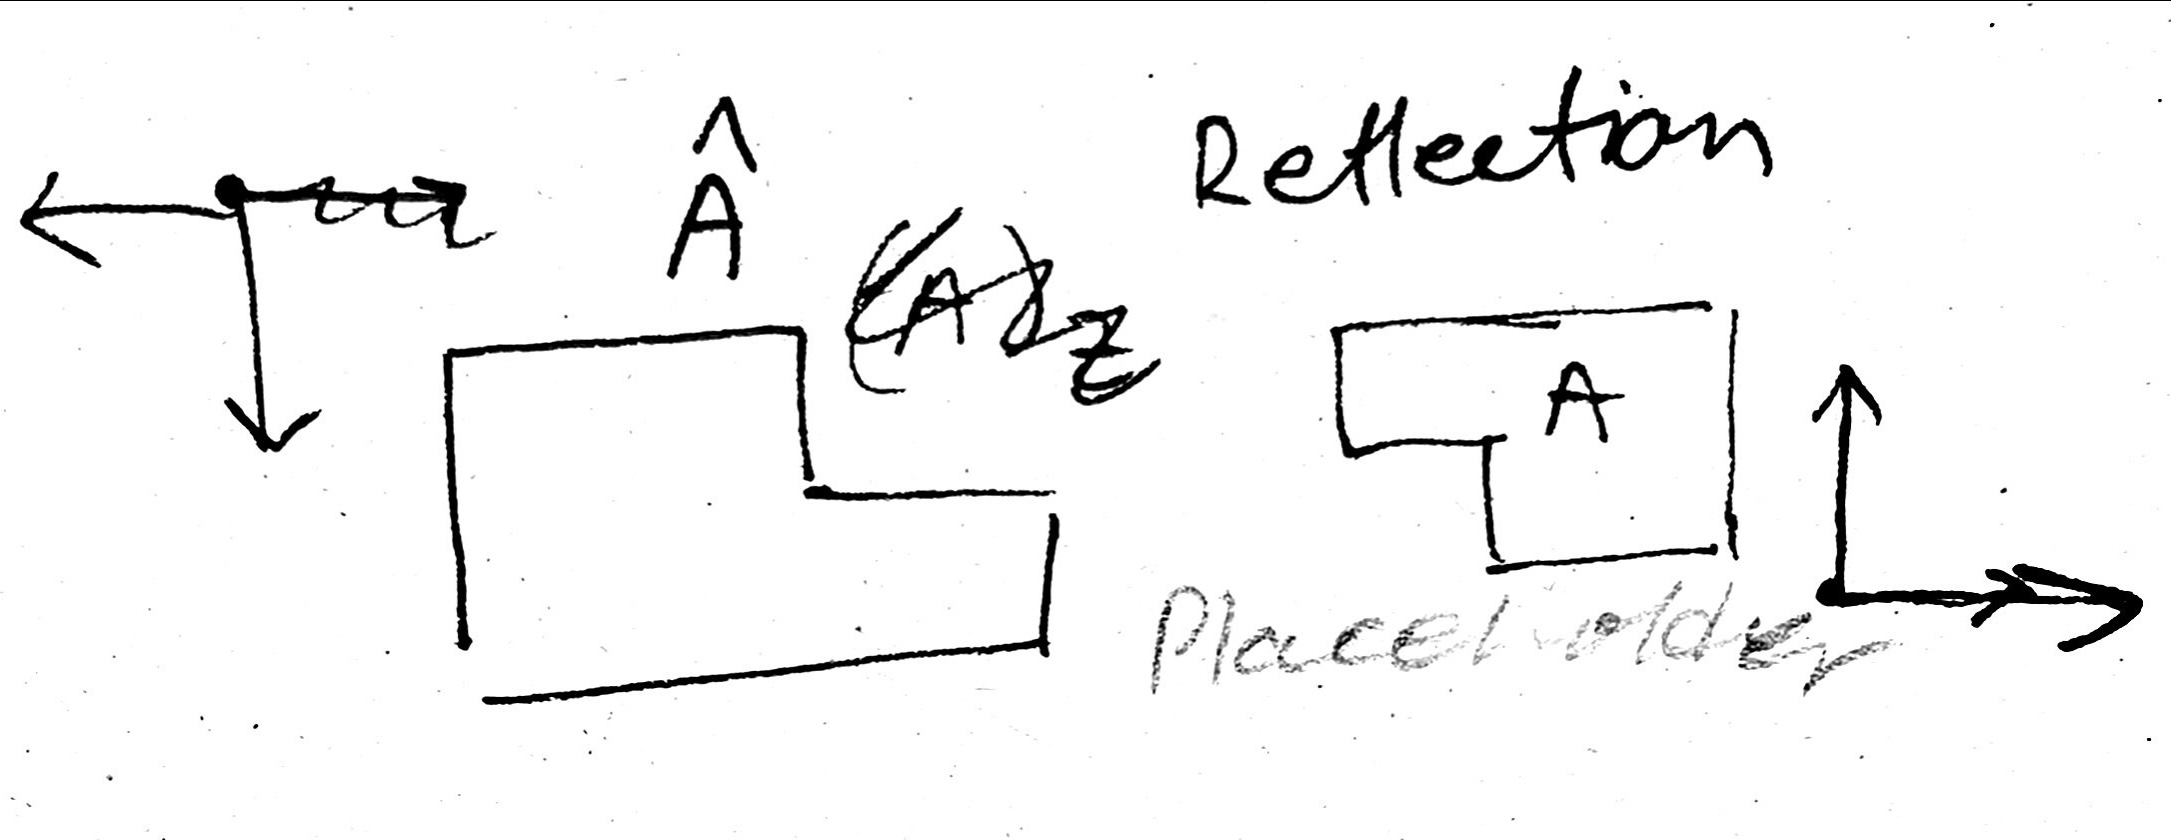
\includegraphics[width=6.3cm]{resources/morph_reflection.jpg}
    \end{center}
    \caption{Morphological reflection} % todo: replace
    \label{fig:morp_refl}
\end{figure}

While manipulating images we commonly have to move parts of the image around.  In principle, a similar operation, called translation, is defined on sets. The formal definition of
moving a set $A$ by some translation vector $z$ is \parencite{gonzalez2002}:
$$(A)_z = \{c | c = a + z\text{ , for } a \in A\}$$
The operation is illustrated in Figure \ref{fig:morph_translation} where the set
$B$ is moved downwards by a vector $z$.
\begin{figure}
    \begin{center}
        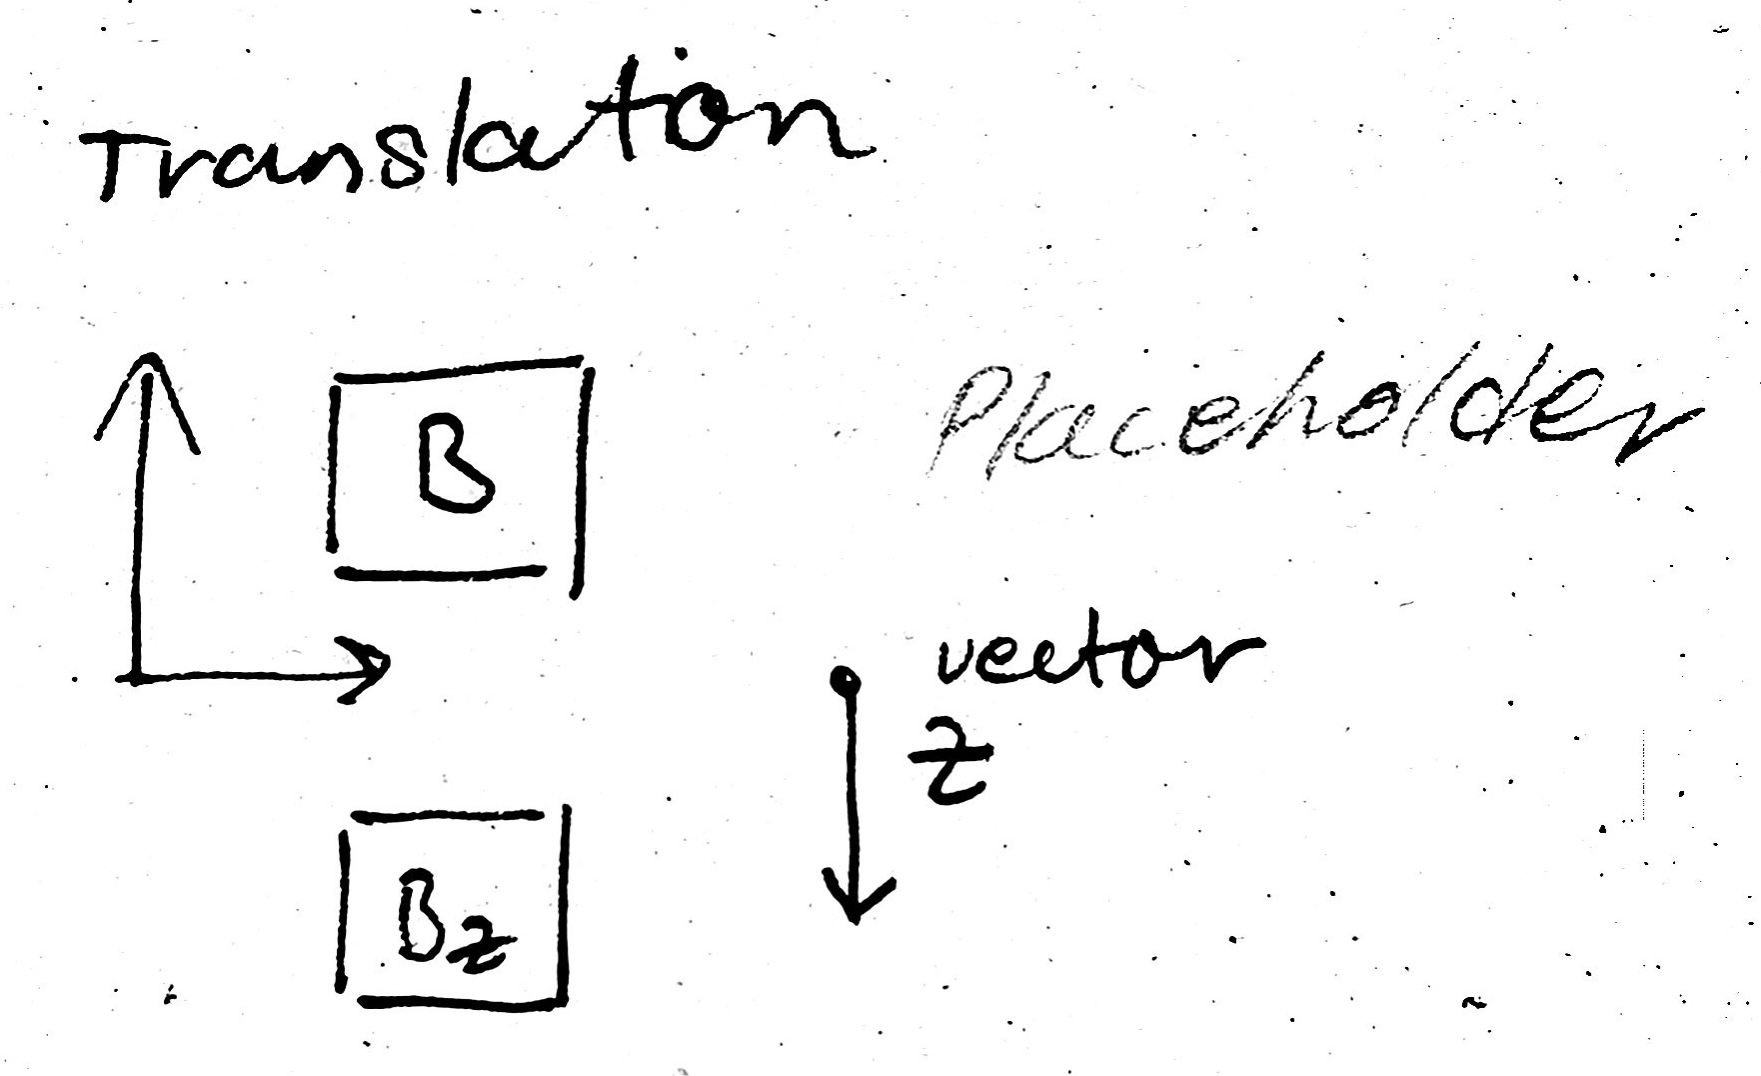
\includegraphics[width=6.3cm]{resources/morph_translation.jpg}
    \end{center}
    \caption{Morphological translation} % todo: Replace
    \label{fig:morph_translation}
\end{figure}

\subsection{Dilation and Erosion}
Now it is possible to properly define two fundamental operations in the field of mathematical morphology, upon which many other operations are built. Both of
these operations include a structural element. A structural element is again a
set, but it can be used to describe how far and in which way the operation will influence the result.


\subsubsection{Dilation}
Intuitively we can think about the dilation
operator as a way to dilate spots inside an image into a bigger space. Formally it is defined
as \parencite{gonzalez2002}
$$A \oplus B = \{z | (\hat{B}_z) \cap A \neq \emptyset\}$$
where $A$ and $B$ are both sets in $\Z^2$.

An example of dilation can be seen in the figure
\ref{fig:morph_dilation}, where two examples are shown. In the first row, we have
a square image with a side length of $d$ and a structuring element whose side length
is a fourth of the original. If we apply the dilation operation on these two
images, we get the one on the right. You can imagine taking the smaller square and
gliding it over the bigger one. If there is an overlap, we can add the centre of
the structural element to the result.

Closer to the mathematical definition, all possible translations are applied to the structural element and if there is an overlap, we add the centre of the structural element to the resulting set.

For example, this operation can be used to join disconnected segments in an
image by choosing a large enough structural element. Its size will depend on the
particular example and does not necessarily have to be of regular size.

\begin{figure}
    \begin{center}
        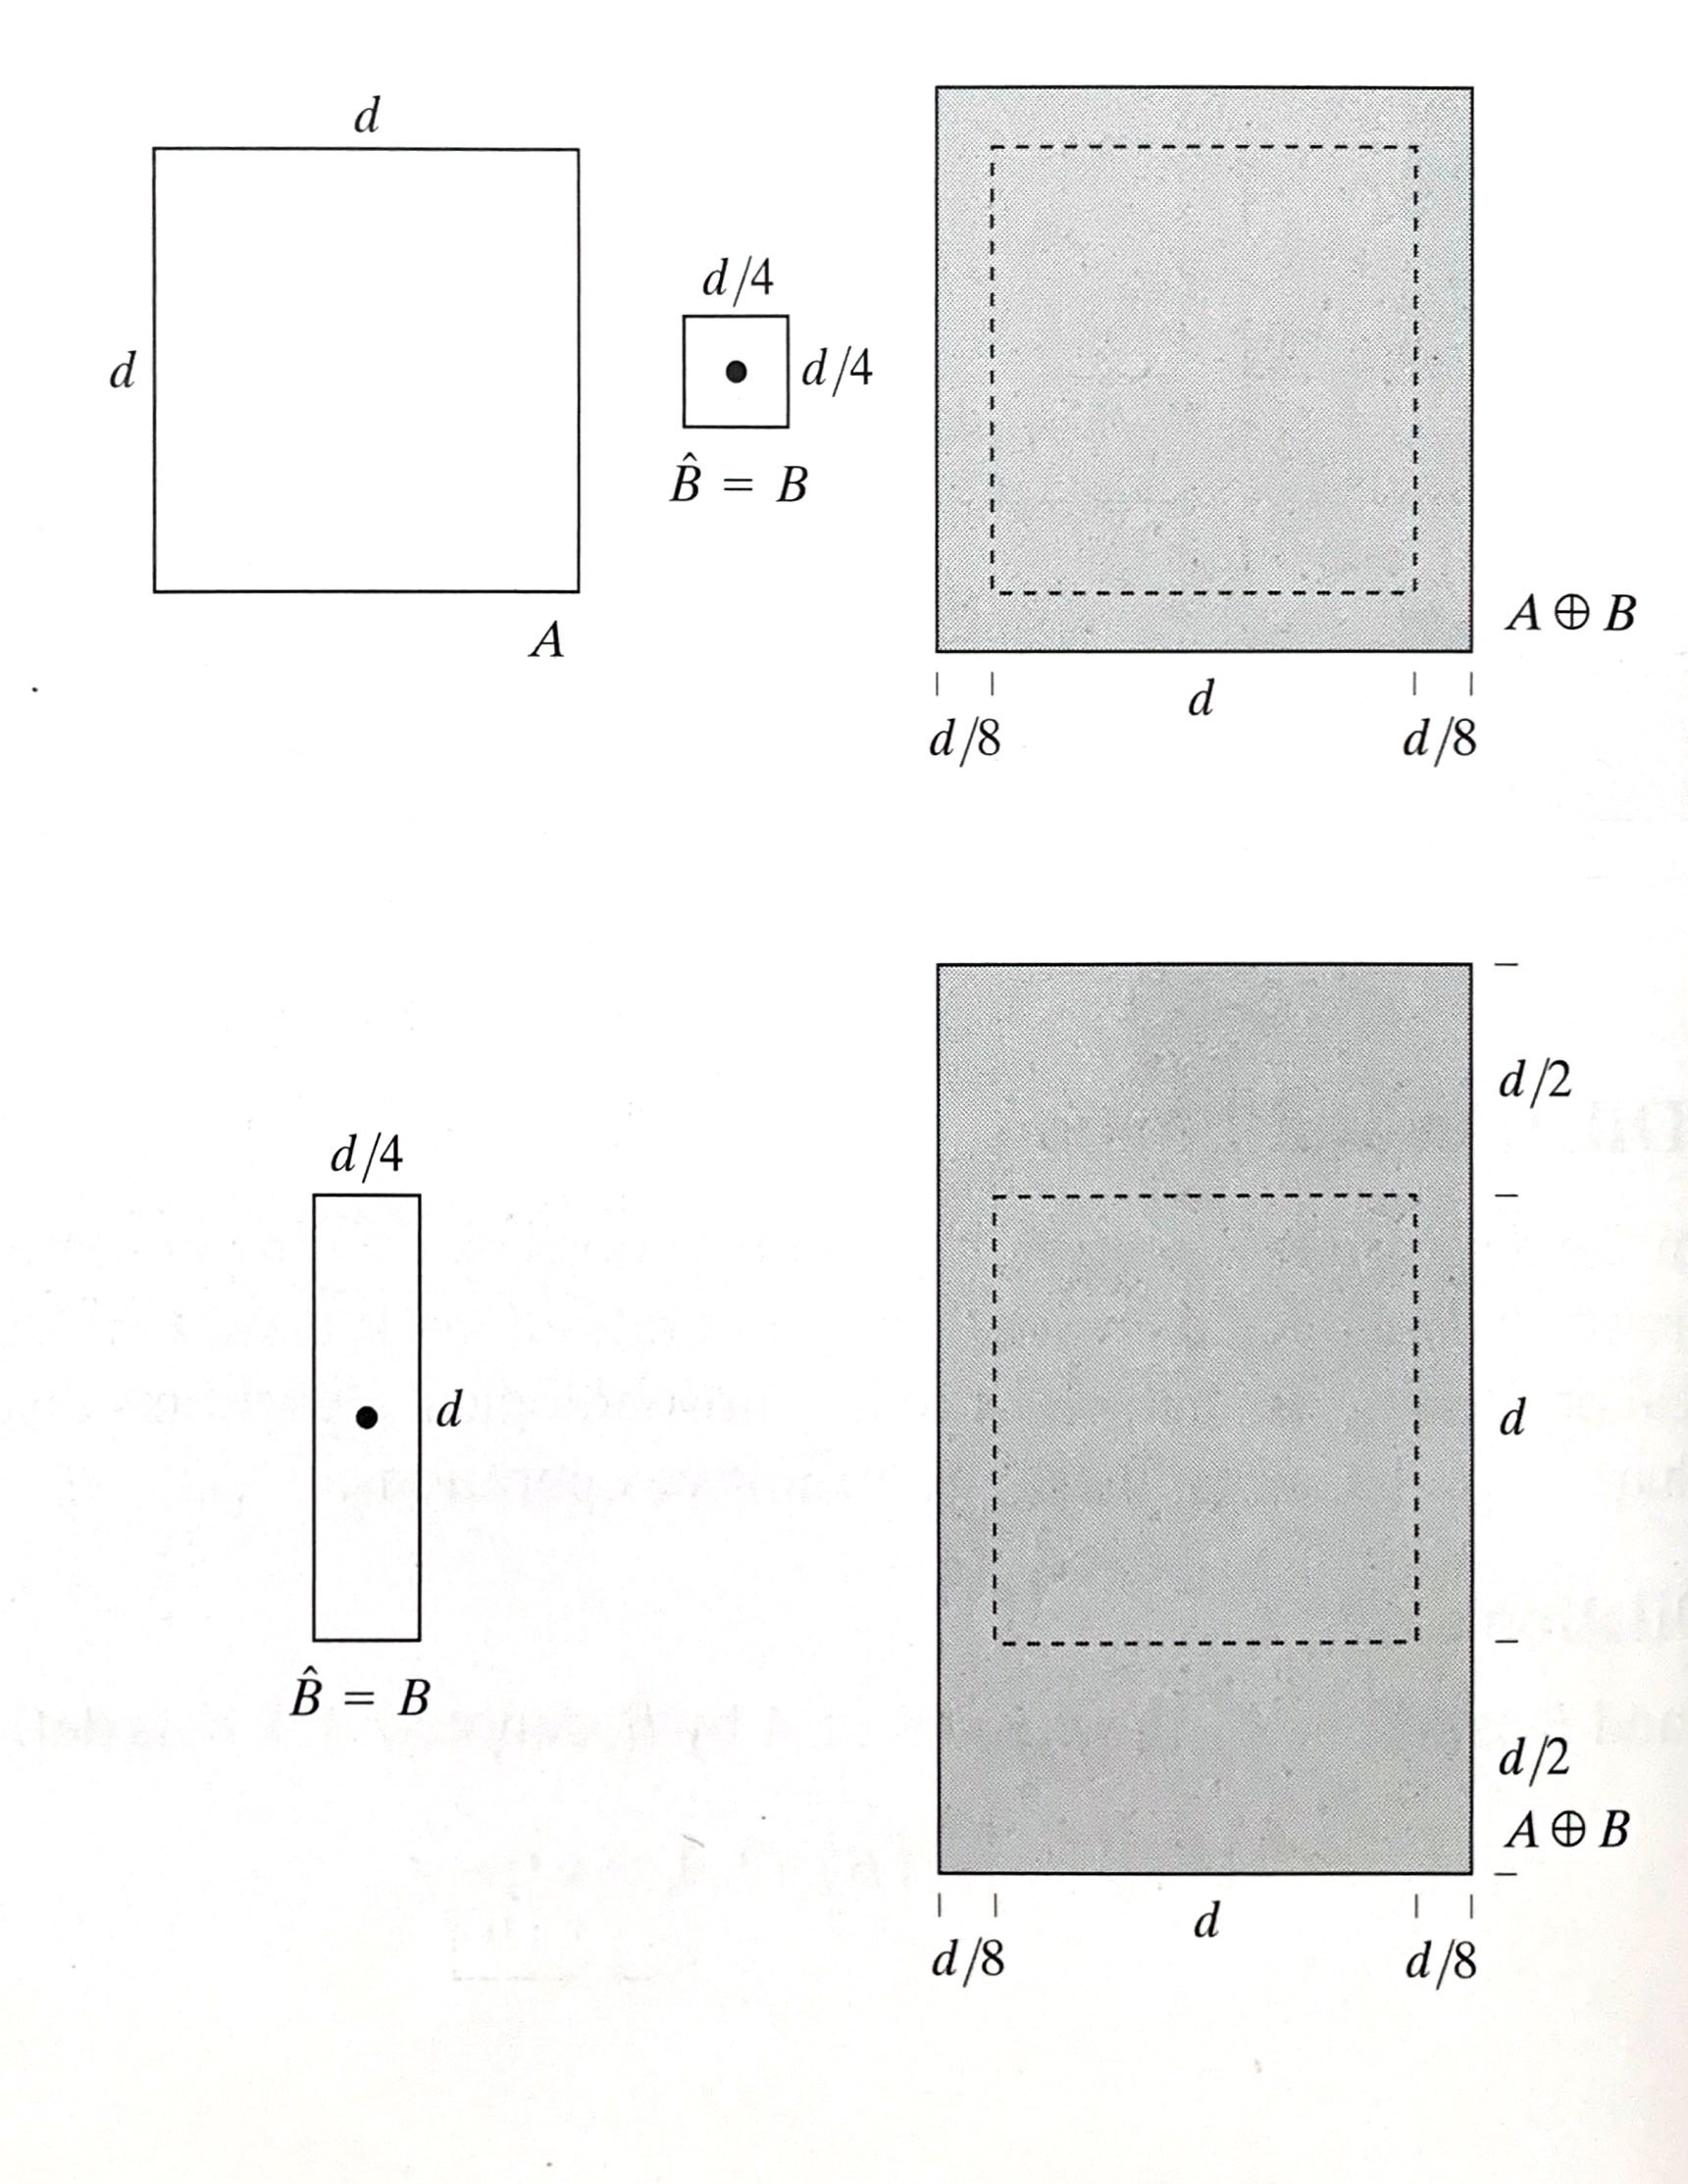
\includegraphics[width=6.3cm]{resources/morph_dilation.jpg}i
    \end{center}
    \caption{Morphological dilation (Gonzalez 2002)} % todo: Replace
    \label{fig:morph_dilation}
\end{figure}

\subsubsection{Erosion}

The next essential operation is erosion. As the name suggests, we use it to erode
parts of the image which we consider unnecessary. An erosion $A \ominus B$ of
two sets $A$ and $B$, both part of $\Z^2$ space, is defined as
\parencite{gonzalez2002}:
$$A \ominus B = \{z | (B)_z \subseteq A\}$$

Again $A$ can be thought of as an image while $B$ can be looked at as a structural
element. In contrast to the dilation operation, we are now looking if the whole
structural element fits inside $A$ as can be seen in the figure
\ref{fig:morph_erosion}. There a smaller structural element is used to cut away
parts of the bigger square.

As opposed to the dilation, we can use erosion to divide lightly connected
segments, and to erase noise and other unwanted disturbances in an image.

While mathematical morphology is a massive topic of interest to many
researchers, here I will only use the aforementioned operations. They can be
further used to define more operations such as binary opening and binary closing
and can be expanded to include grayscale images; however, I will not be using or covering
them in my thesis.

\begin{figure}
    \begin{center}
        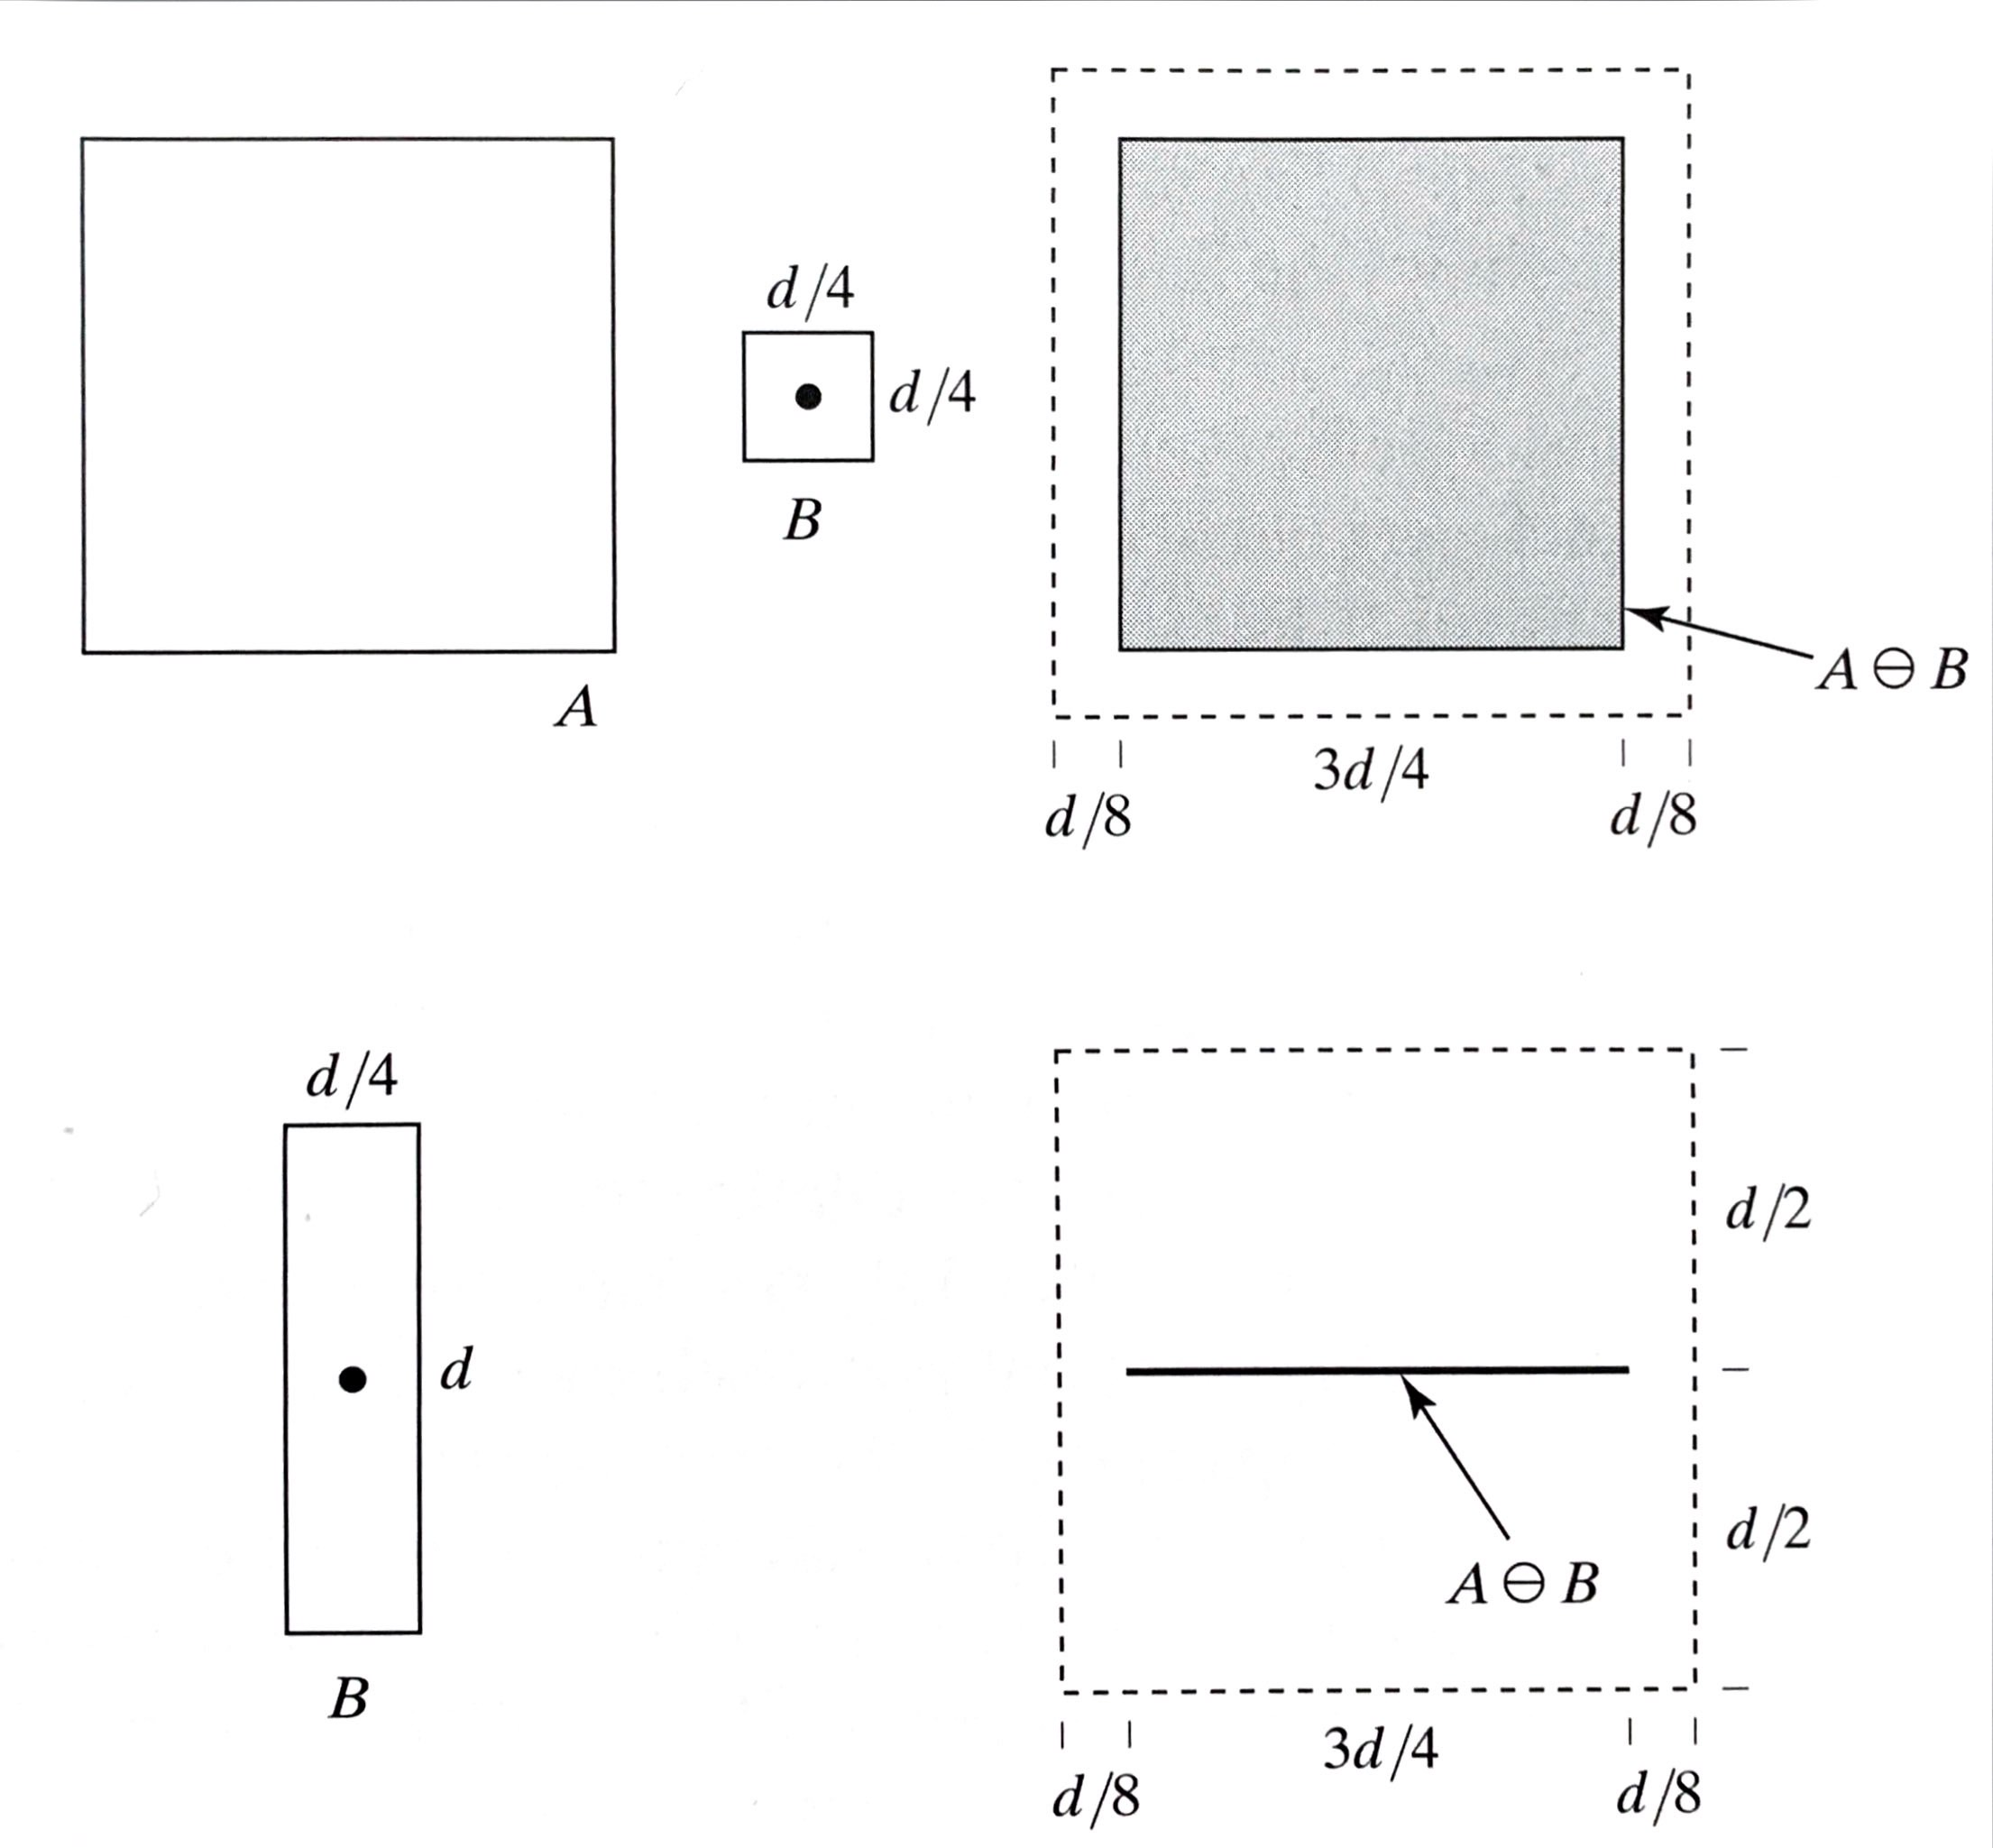
\includegraphics[width=6.3cm]{resources/morph_erosion.jpg}
    \end{center}
    \caption{Morphological erosion (Gonzalez 2002)} % todo: Replace
    \label{fig:morph_erosion}
\end{figure}

\section{Segmentation}

\chapter{Image data}

The image data --- of organoids of mammary glands in mice --- was acquired using
a fluorescence microscope. The original data was captured in 2011 by a group of
researchers at (\textbf{TODO}) faculty. The captured specimen is around 500
microns by 500 microns by 80 microns big with a resolution of around 4.3 microns
per pixel.

In fluorescence microscopy, researchers are able to stain specific structures in
their specimen so that wanted structures reemit light when the proper wavelength
is shined upon them. This allows them to capture the density of studied proteins
inside the specimen. In this particular case, the researchers captured the
density of six different proteins, of which two are part of membranes, while the
other four are primarily located inside the cell's nuclei.

The data, totalling around 576 GB, consists of 12 different time steps, where
each step has a size of 1920x1920x388 pixels and six different channels. The
data is stored in numerous TIFF files, and every channel contains grayscale data
with 16 bits per pixel. All visualisations of the data had to be manually
preprocessed before including them in this thesis. Otherwise, it would be hard
to see anything.

\begin{figure}
    \begin{center}
        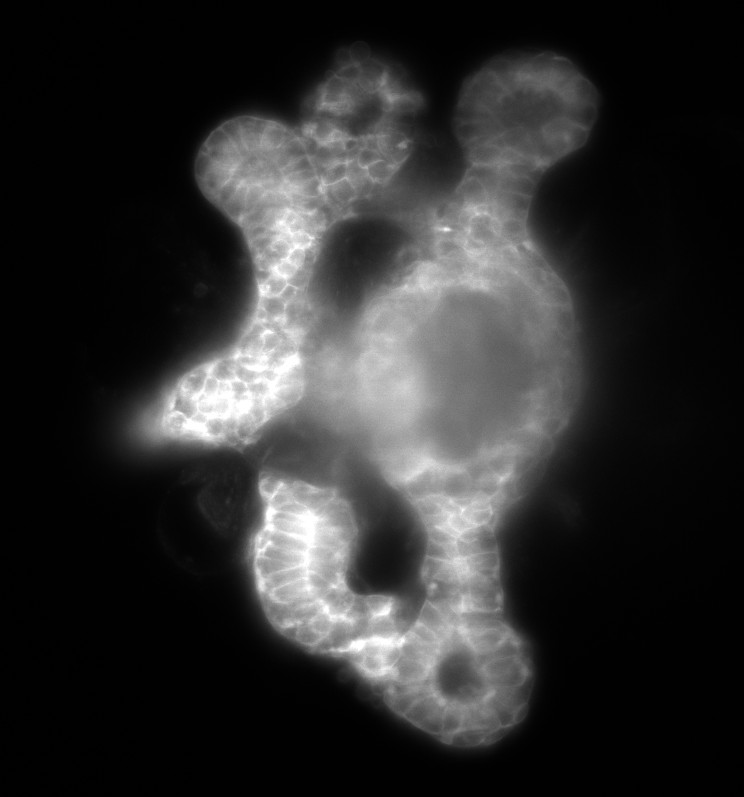
\includegraphics[width=6.3cm]{resources/C3-t006-200-scaled.jpg}
        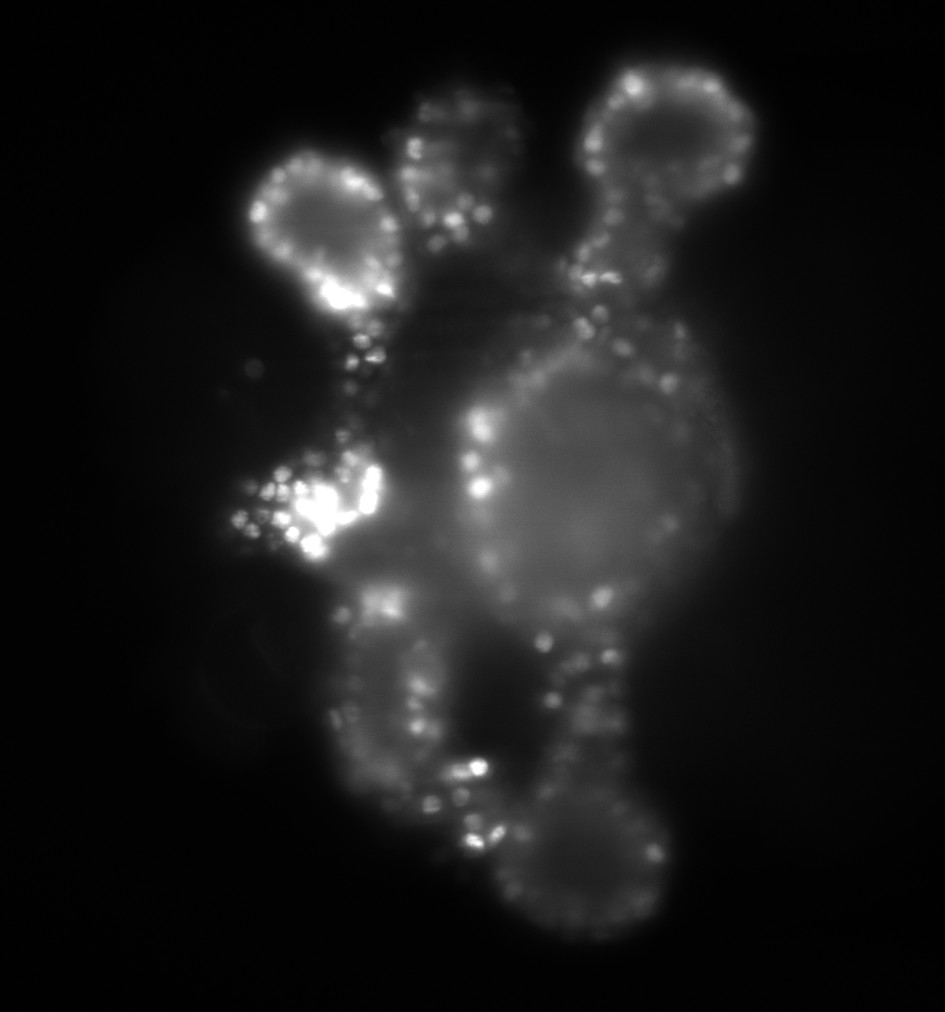
\includegraphics[width=6.3cm]{resources/C2-t006-200-scaled.jpg}
    \end{center}
    \caption{Membraine stained channel and nucleus stained channel}
    \label{fig:data_example}
\end{figure}
In the Figure \ref{fig:data_example} a single slice of the data was taken from
two channels. They are from the same moment of time and from the same place. On
the left one of the proteins forming the membrane is showcased while on the right a
different protein mostly located in nuclei is shown.

\section{Problems with the dataset}

The size of the data and the inherent problems of fluorescence microscopy
provide the main issues in analyzing the data. It is very time consuming to
analyse the whole data set; therefore, all work was done on much smaller slices
of the data. Interesting regions with well lit

\subsection{Noise}

The first problem with the data set is the quality. In most places, the noise is
too strong to try to use it in any analysis.

In the membrane channel, two main problems can be seen seen. To begin, most
membranes do not form connected segments, instead, a part the cell's membrane is
usually missing or it is joined with the neighbouring cell's membrane as can be
seen on the Figure \textbf{TODO}. This complicates the analysis, as different
regions may require different filters to be properly preprocessed. Moreover,
this makes the edge detection much harder, since it relies on the magnitude of
gradient of the image.

Another issue is that the light gets scattred inside the organoid as can be seen
on Figure \textbf{TODO}. That means that it is possible to analyze only the
outer most layers of cells of the organoid.

The protein channel comes with its own set of problems, some of them different.
It is still true, that the sharpest data comes, again, from the outermost layer
of the organoid, limiting the amount of usable data. Another issue is that the
individual cells are sometimes quite fuzzy, which makes it hard to decide, where
exactly the cells ends, or if they are multiple cells.
% todo: reword

\subsection{Size}

The size of the dataset poses the second problem, as it would be computationaly
expensive to try to process the whole data set at once; however a lot of the
data is either unusable or of no interest. In most instances, the data is
predominantly composed of the background, and at several moments in time, no
specimen can be seen; therefore, to reduce the computational demands further,
only specific regions of interest were manually selected to create the final
data set. In the end, the reduced data set is only a few dozen megabytes large.

\chapter{The developed segmentation method}

TODO: introductory paragraph

\section{Overview/Goals}

High level overview of the process.

\section{Membrane channel}

Steps inside the membrane channel: watershed, thresholding, denoising, edge
detection

\section{Protein channel}

Steps inside the protein channel: thresholding, denoising

\end{document}
